%%%%%%%%%%%%%%%%%%%%%%%%%%%%%%%%%%%%%%%%%%%%%%%%%%%%%%%%%%%
% 
%%%%%%%%%%%%%%%%%%%%%%%%%%%%%%%%%%%%%%%%%%%%%%%%%%%%%%%%%%%


%%%%%%%%%%%%%%%%%%%%%%%%%%%%%%%%%%%%%%%%%%%%%%%%%%%%%%%%%%%
%%%%%%%%%%%%%%%%%%%%%%%%%%%%%%%%%%%%%%%%%%%%%%%%%%%%%%%%%%%
\section{Notation and Terminology}
%%%%%%%%%%%%%%%%%%%%%%%%%%%%%%%%%%%%%%%%%%%%%%%%%%%%%%%%%%%
%%%%%%%%%%%%%%%%%%%%%%%%%%%%%%%%%%%%%%%%%%%%%%%%%%%%%%%%%%%


%%%%%%%%%%%%%%%%%%%%%%%%%%%%%%%%%%%%%%%%%%%%%%%%%%%%%%%%%%%
\subsection{Measure Theory 101}
%%%%%%%%%%%%%%%%%%%%%%%%%%%%%%%%%%%%%%%%%%%%%%%%%%%%%%%%%%%

\begin{frame}[t]
%\vskip 25pt
\centering
\begin{figure}
\centering

The one with the background on inverse problems.

\end{figure}

\end{frame}

%%%%%%%%%%%%%%%%%%%%%%%%%%%%%%%%%%%%%%%%%%%%%%%%%%%%%%%%%%
\begin{frame}{The QoI Map Relates Inputs and Outputs}

\only<1>{

\begin{figure}[h]
	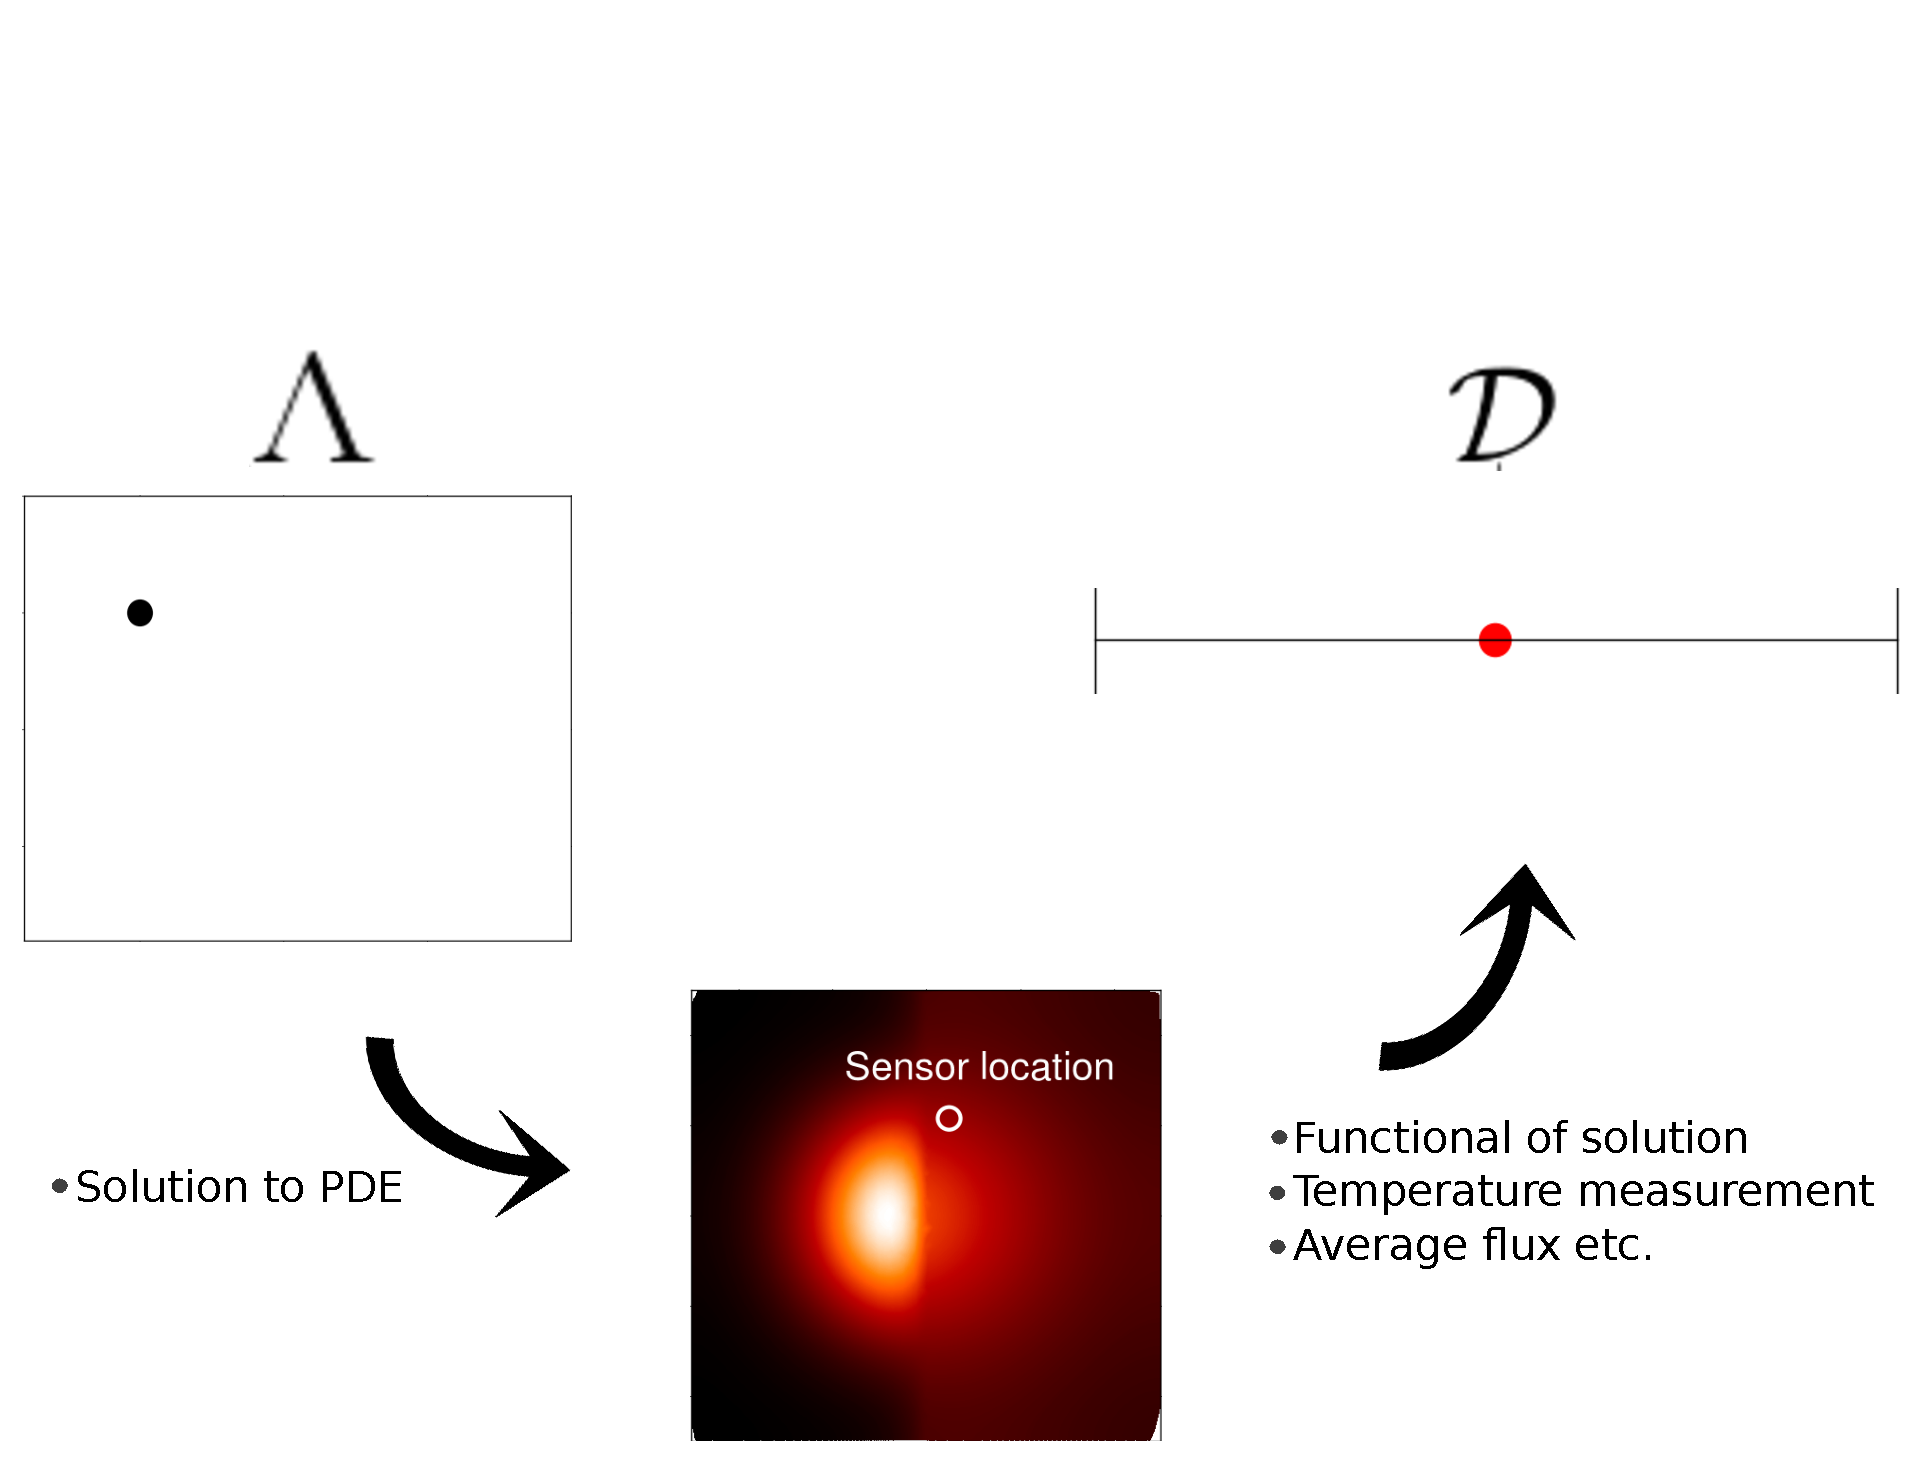
\includegraphics[width=0.85\textwidth]{./figures/threelevels/schematic_lambda_solution_data.pdf}
\end{figure}

}

\only<2>{

\begin{figure}[h]
	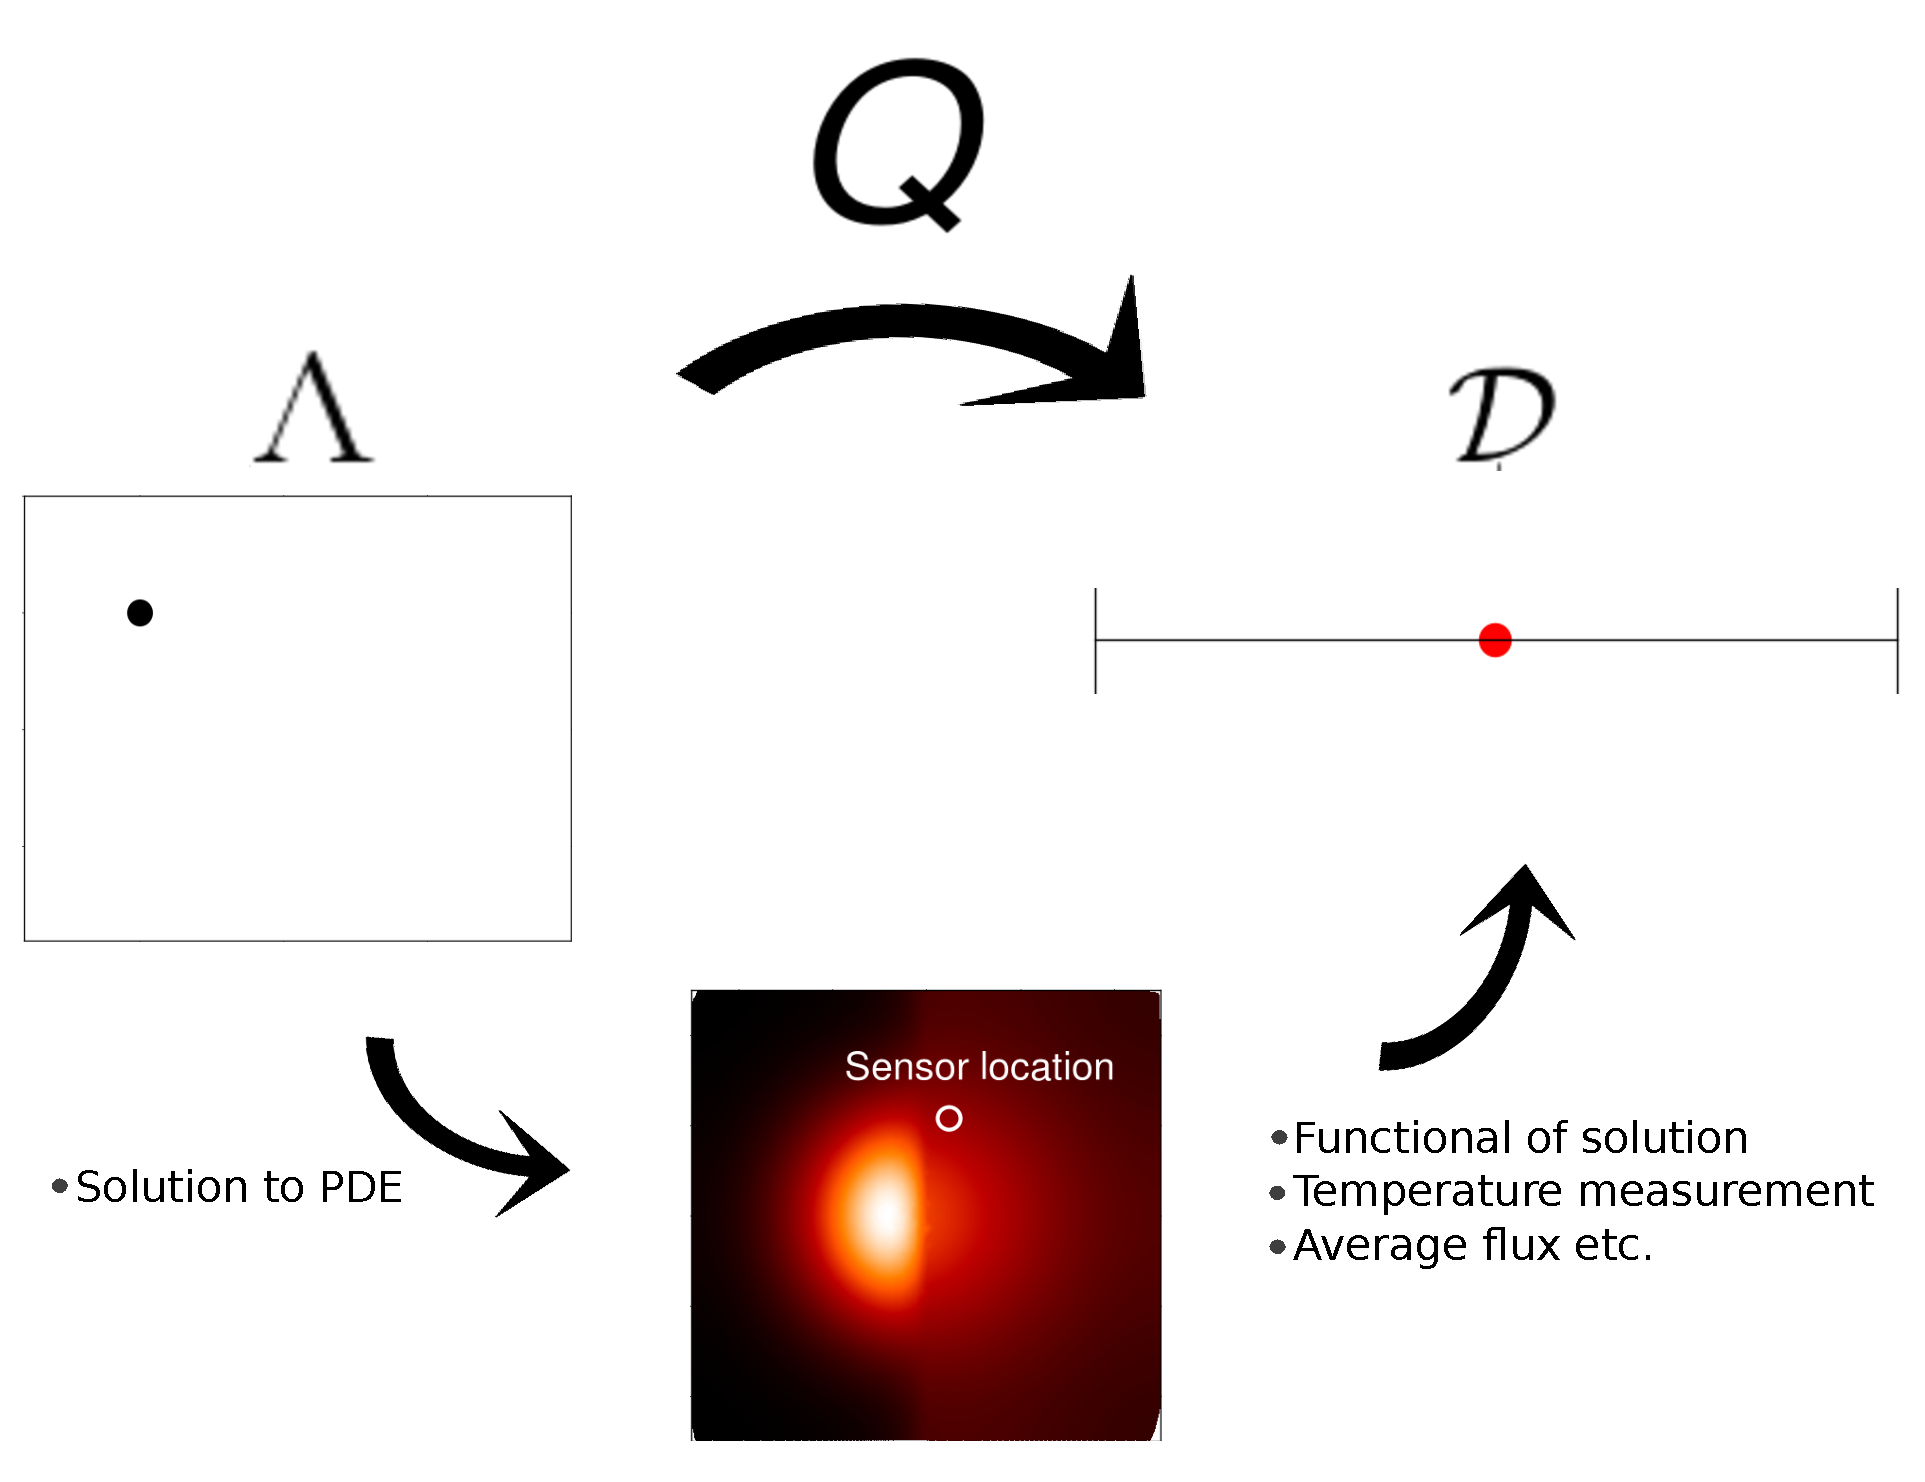
\includegraphics[width=0.85\textwidth]{./figures/threelevels/schematic_lambda_data.pdf}
\end{figure}

}

\only<3>{

\begin{figure}[h]
	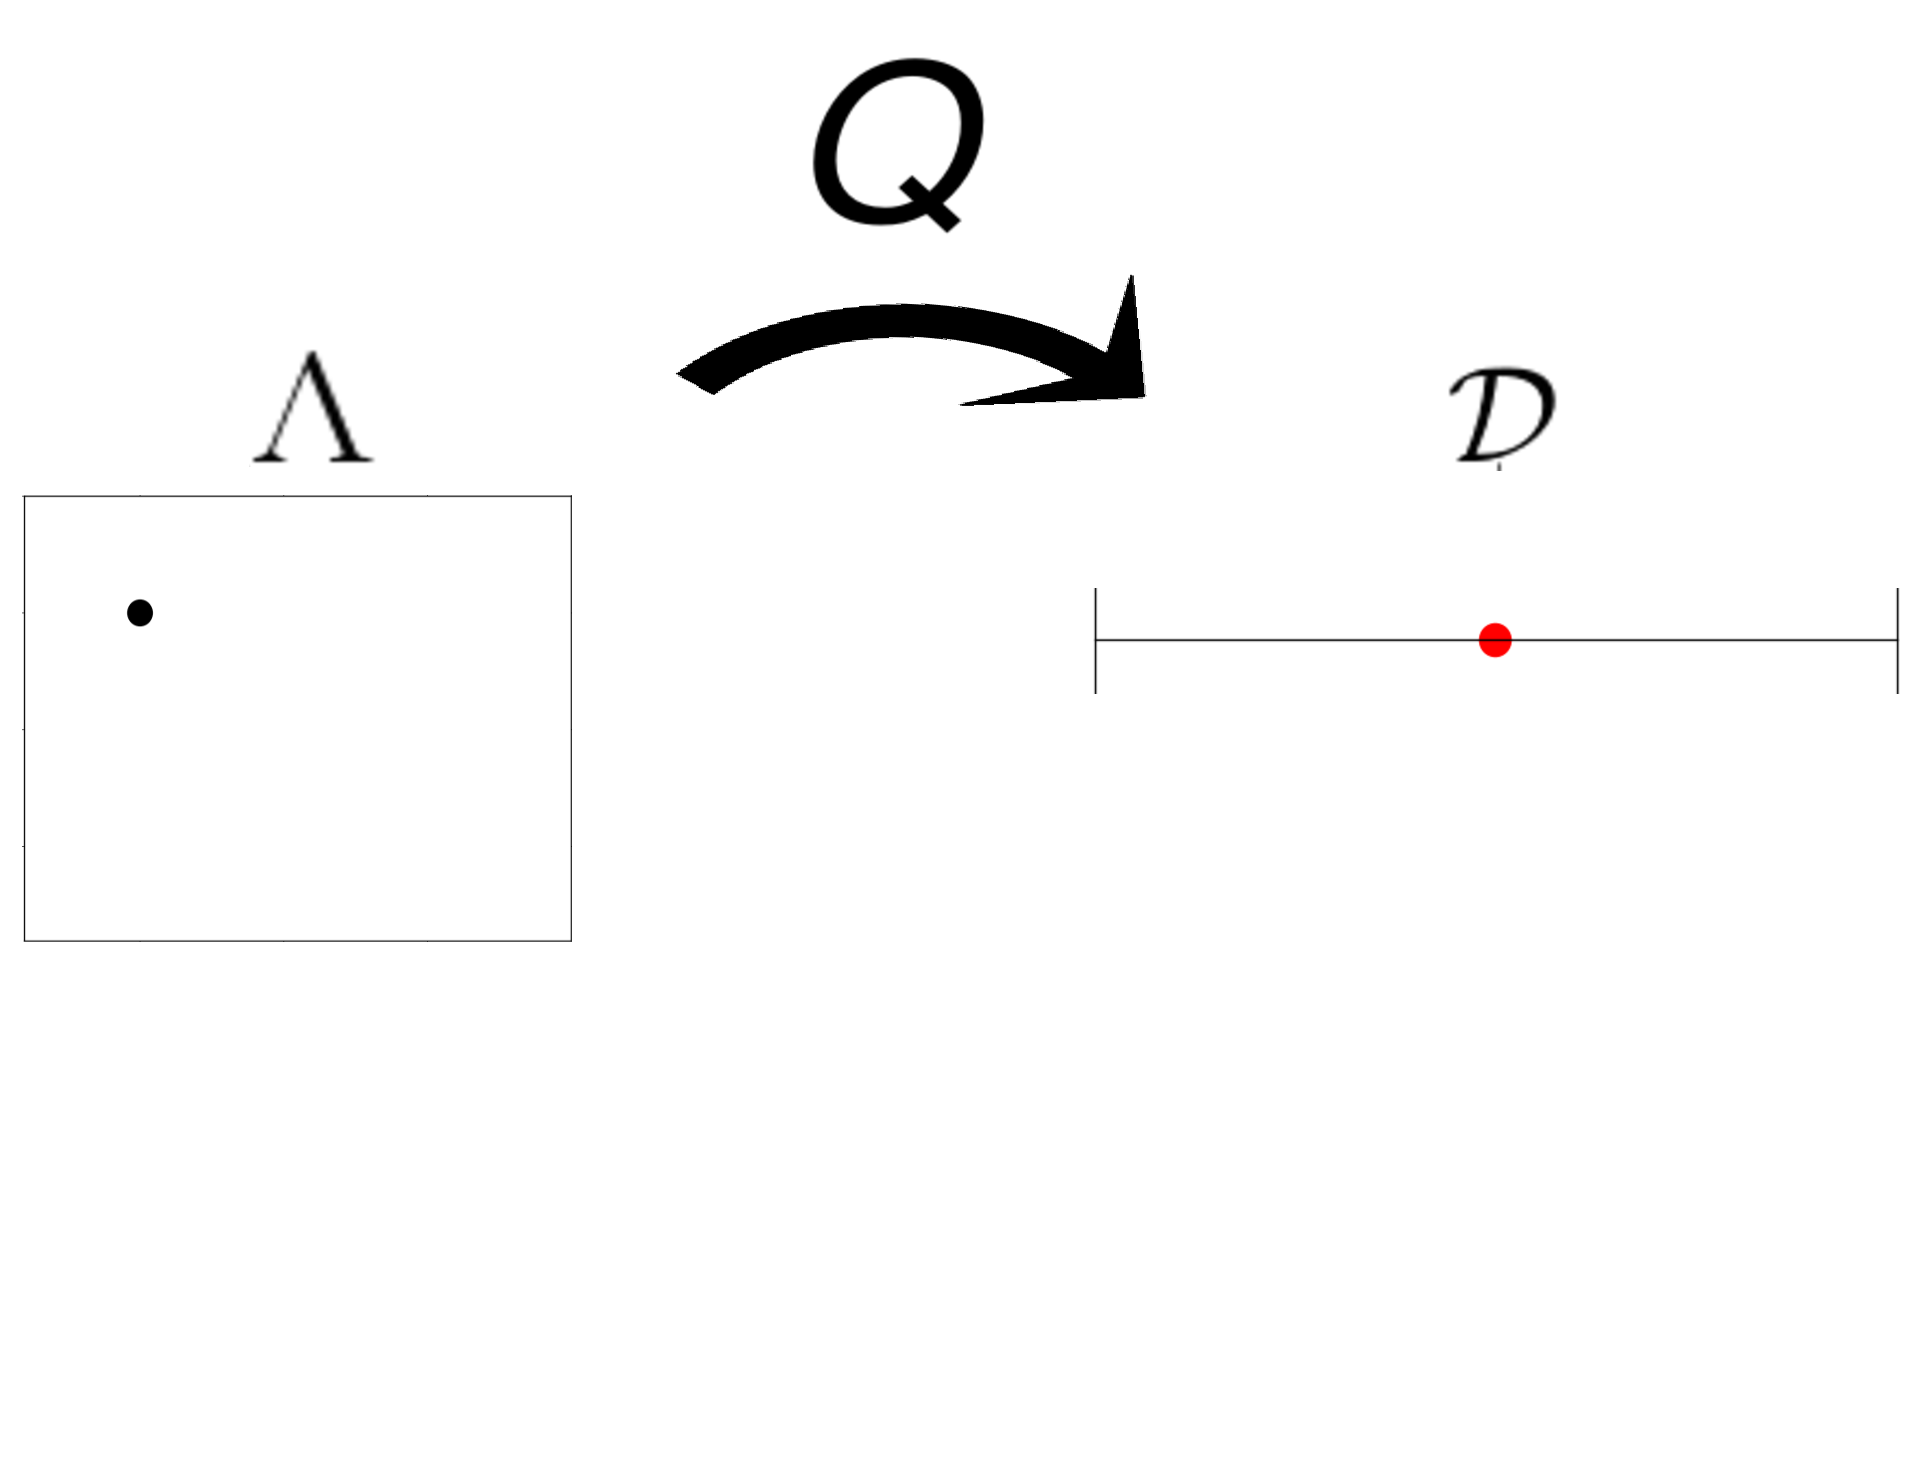
\includegraphics[width=0.85\textwidth]{./figures/threelevels/schematic_lambda_data_level1.pdf}
\end{figure}

}

\end{frame}

%%%%%%%%%%%%%%%%%%%%%%%%%%%%%%%%%%%%%%%%%%%%%%%%%%%%%%%%%%
\begin{frame}{A Forward UQ Problem}

\begin{figure}[h]
	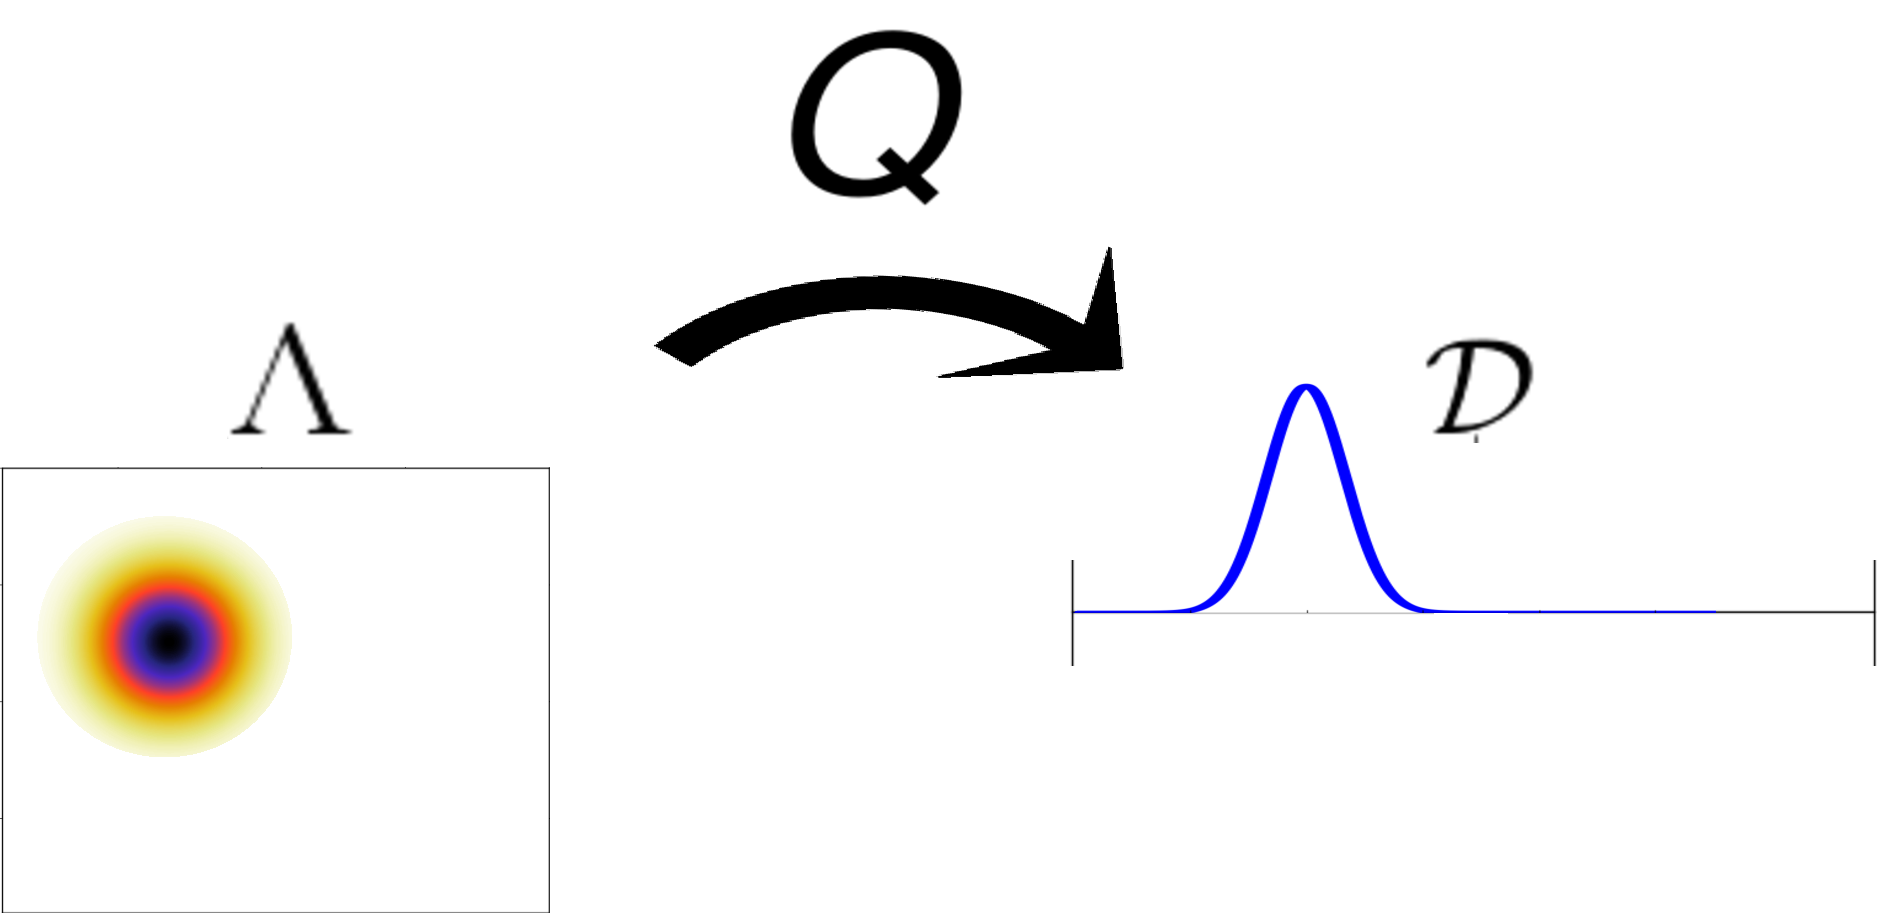
\includegraphics[width=0.85\textwidth]{./figures/threelevels/schematic_lambda_data_level3.pdf}
\end{figure}

{We denote the measurable spaces of parameters and data on the QoI as $(\pspace,\pborel)$ and $(\dspace,\dborel)$, respectively.}
\bigskip

\tdeepred{Given some prior density $\initial$ on $(\pspace,\pborel)$, we let $\predicted$ denote the push-forward of this density on $(\dspace,\dborel)$.}

\end{frame}

%%%%%%%%%%%%%%%%%%%%%%%%%%%%%%%%%%%%%%%%%%%%%%%%%%%%%%%%%%
\begin{frame}{The Inverse QoI Map}

\begin{figure}[h]
	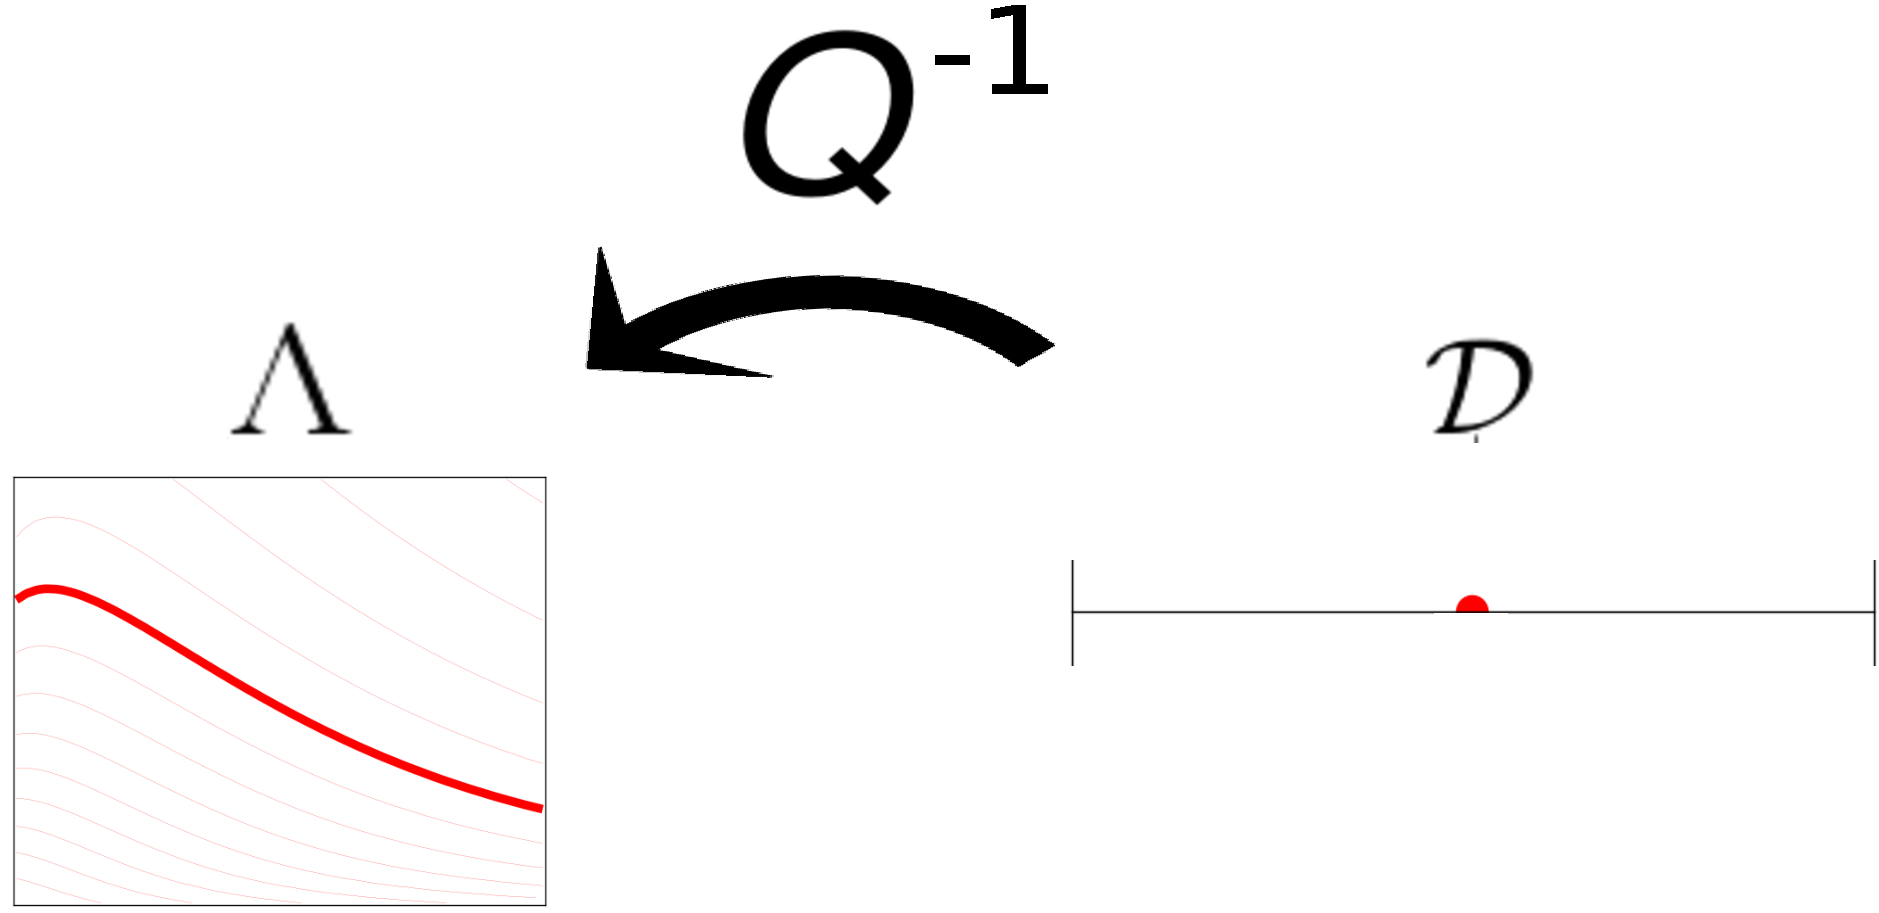
\includegraphics[width=0.85\textwidth]{./figures/threelevels/schematic_data_lambda_level1.pdf}
\end{figure}

\end{frame}

%%%%%%%%%%%%%%%%%%%%%%%%%%%%%%%%%%%%%%%%%%%%%%%%%%%%%%%%%%
\begin{frame}{An Inverse UQ Problem}

\begin{figure}[h]
	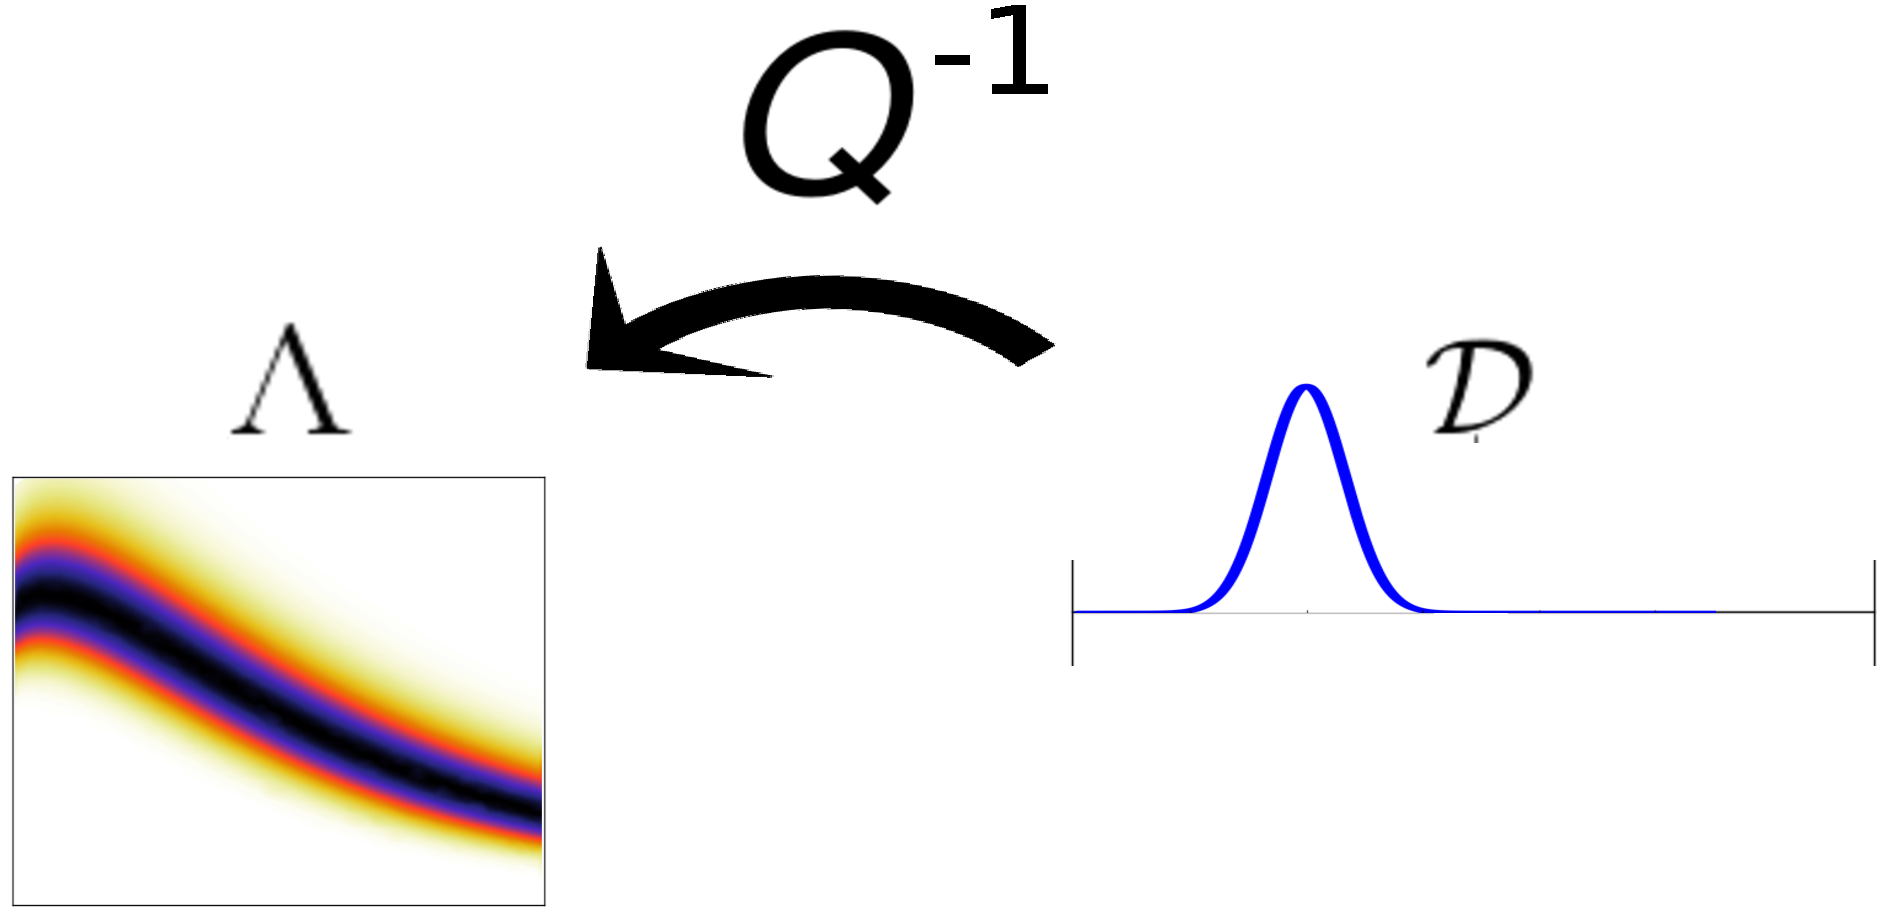
\includegraphics[width=0.85\textwidth]{./figures/threelevels/schematic_data_lambda_level3.pdf}
\end{figure}

\tdeepred{Given $\obs$ on $(\dspace,\dborel)$, we let $\predicted$ denote the pullback (consistent) density on $(\pspace,\pborel)$.}

\end{frame}



\subsection{The Stochastic Inverse Problem}
%%%%%%%%%%%%%%%%%%%%%%%%%%%%%%%%%%%%%%%%%%%%%%%%%%%%%%%%%%
\begin{frame}[t]

\begin{figure}
\centering
	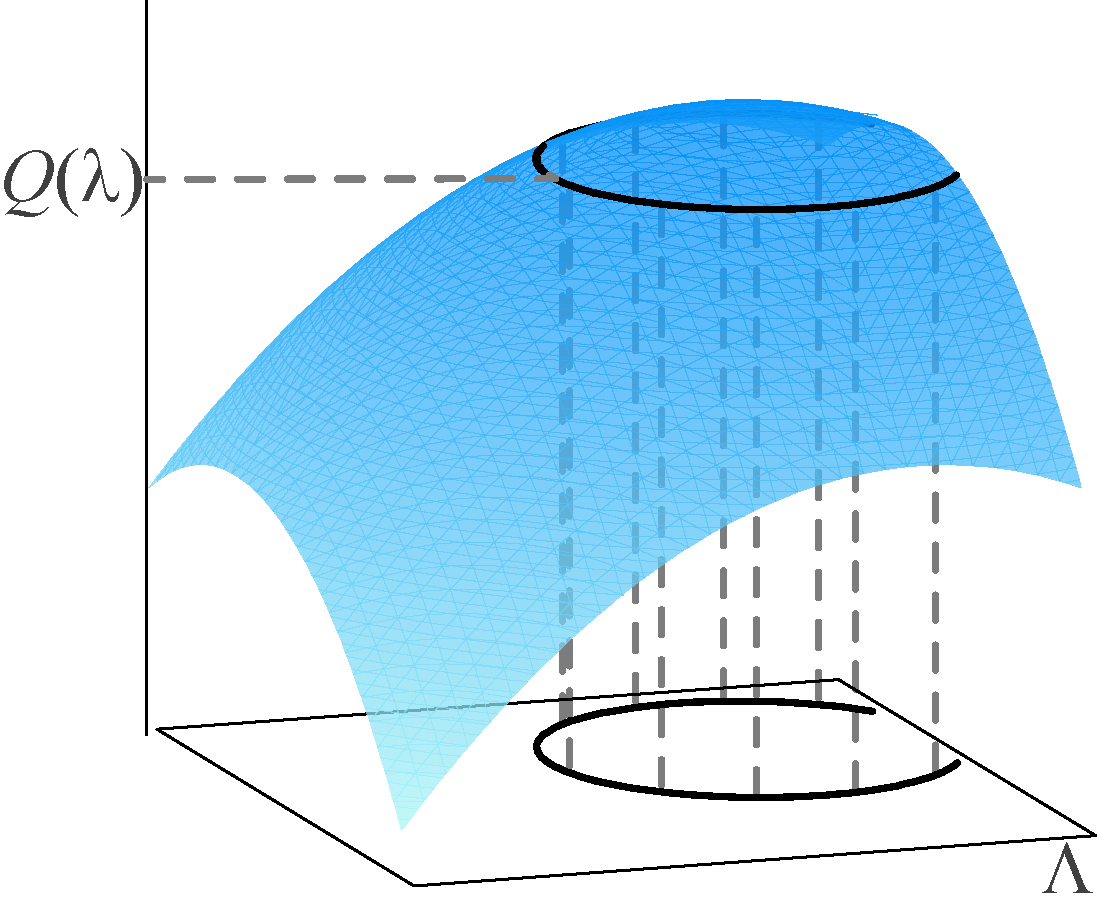
\includegraphics[width=.65\textwidth]{images/illustration1.pdf}<1>
	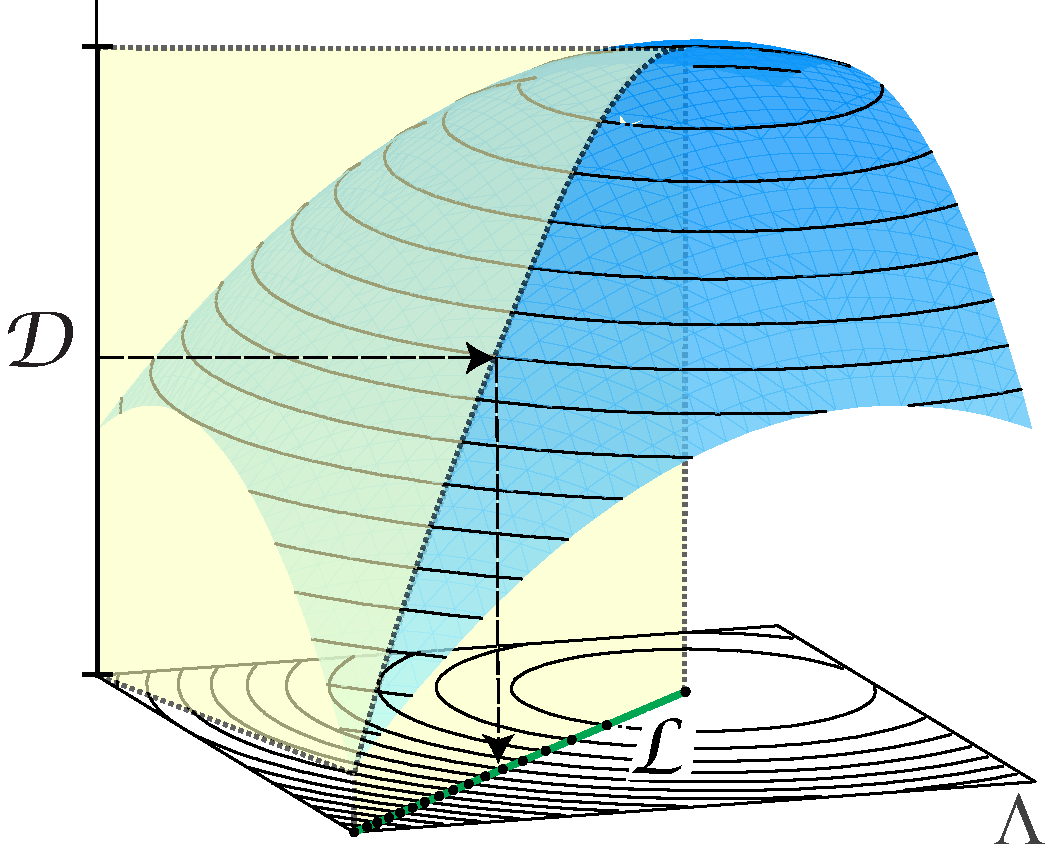
\includegraphics[width=.65\textwidth]{images/illustration2.pdf}<2>
	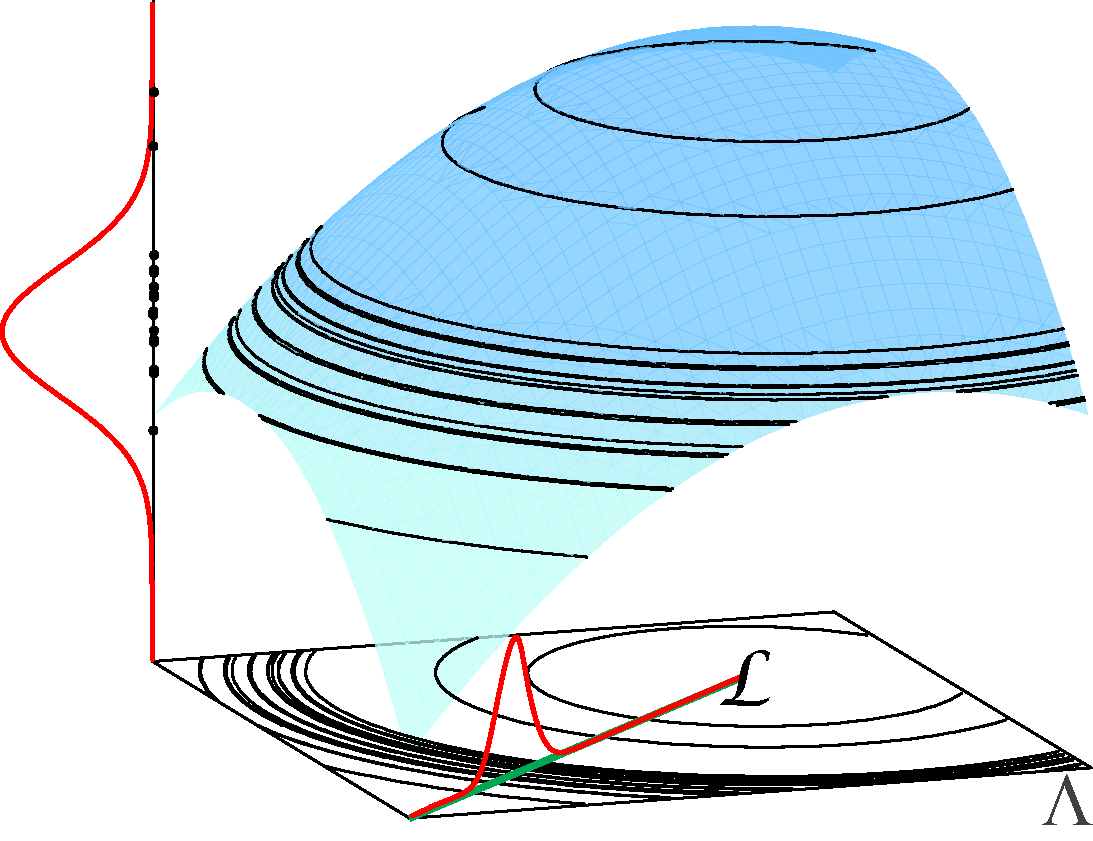
\includegraphics[width=.7\textwidth]{images/illustration3.pdf}<3>
\end{figure}
\begin{center}
{\scriptsize Figure adopted from \cite{BET14+} and used with permission}
\end{center}
\end{frame}

%%%%%%%%%%%%%%%%%%%%%%%%%%%%%%%%%%%%%%%%%%%%%%%%%%%%%%%%%%
\begin{frame}[t]

\begin{figure}
\centering
	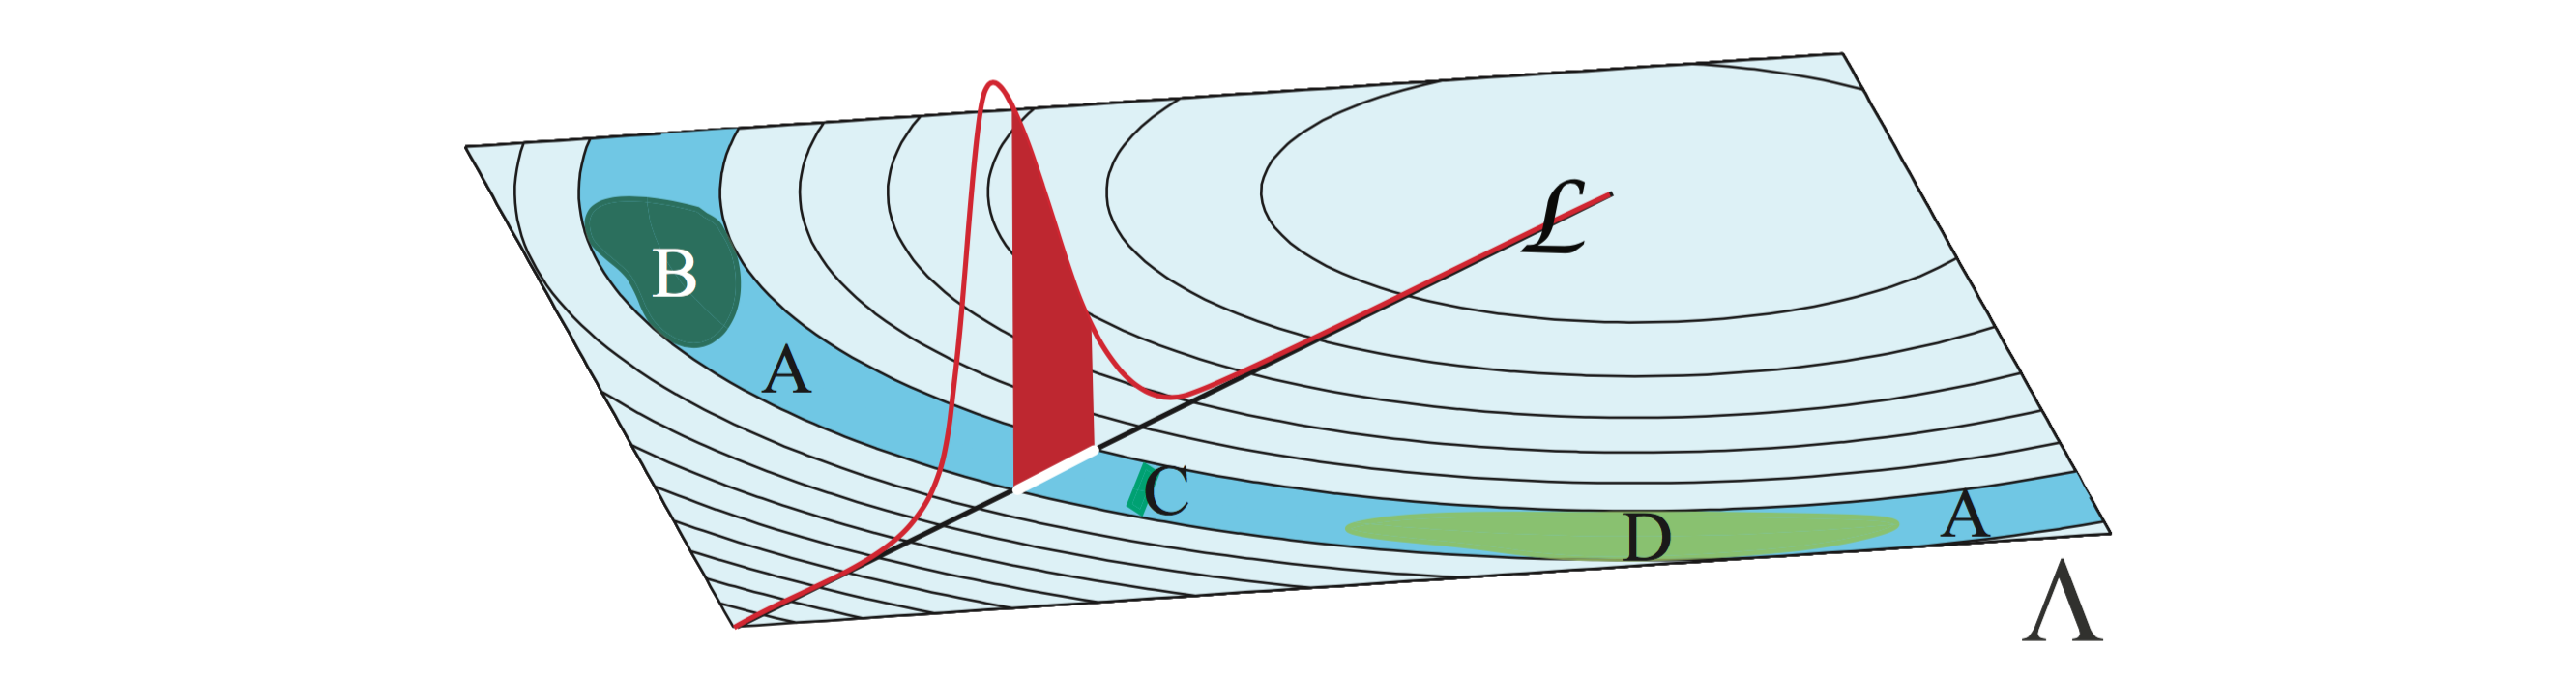
\includegraphics[width=1\textwidth]{images/troy_mt3contour.png}
\end{figure}
\begin{center}

{\scriptsize Figure adopted from \cite{BET14+} and used with permission}

\tdeepred{Key Question:} Distinguish (assign probability to) events that belong to same contour.
\end{center}
\end{frame}

\subsection{Problem Formulation and Solution}
%%%%%%%%%%%%%%%%%%%%%%%%%%%%%%%%%%%%%%%%%%%%%%%%%%%%%%%%%%%
\begin{frame}

\begin{defn}[Stochastic Forward Problem (SFP)]\label{defn:forward-problem}
  Given a probability measure $\PP_\pspace$ on $(\pspace, \pborel)$, and QoI map $\qoi$, the \emph{stochastic forward problem} is to determine a measure, $\PP_\dspace$, on $(\dspace, \dborel)$ that satisfies
  \begin{equation}\label{eq:forward-problem}
    \PP_\dspace (E) = \PP_\pspace \left ( \qoi^{-1}(E) \right ), \; \forall \; E \in \dborel.
  \end{equation}
\end{defn}

\end{frame}

\begin{frame}

\begin{defn}[Stochastic Forward Problem (SFP)]\label{defn:forward-problem}
  Given a probability measure $\PP_\pspace$ on $(\pspace, \pborel)$, and QoI map $\qoi$, the \emph{stochastic forward problem} is to determine a measure, $\PP_\dspace$, on $(\dspace, \dborel)$ that satisfies
  \begin{equation}\label{eq:forward-problem}
    \PP_\dspace (E) = \PP_\pspace \left ( \qoi^{-1}(E) \right ), \; \forall \; E \in \dborel.
  \end{equation}
\end{defn}

\begin{defn}[Stochastic Inverse Problem (SIP)]\label{defn:inverse-problem}
Given a probability measure, $\PP_\dspace$, on $(\dspace, \dborel)$ the \emph{stochastic inverse problem} is to determine a probability measure, $\PP_\pspace$, on $(\pspace, \pborel)$ satisfying
\begin{equation}\label{eq:inverse-problem}
\PP_\pspace (\qoi^{-1}(E)) = \PP_\dspace(E), \; \forall \; E \in \mathcal{B}_\dspace.
\end{equation}
\end{defn}

Equation~\eqref{eq:inverse-problem} is referred to as the \emph{consistency condition}.

\end{frame}


%%%%%%%%%%%%%%%%%%%%%%%%%%%%%%%%%%%%%%%%%%%%%%%%%%%%%%%%%%%
\begin{frame}

\begin{defn}[Consistent Solution and Density]\label{defn:consistent-solution}
  If $\PP_\pspace$ or $\PP_\dspace$ absolutely continuous w.r.t $\pmeas$ or $\dmeas$, resp, then we write

  \begin{equation*}
    \pp_\pspace := \frac{d\PP_\pspace}{d\pmeas} \;\text{ or }\; \pp_\dspace := \frac{d\PP_\dspace}{d\dmeas}
  \end{equation*}
  to denote the Radon-Nikodym derivatives of $\PP_\pspace$ and $\PP_\dspace$, resp.
  \bigskip

  In such a case, we can rewrite \eqref{eq:forward-problem} and \eqref{eq:inverse-problem} using these pdfs:
  \begin{equation*}
  \PP_\pspace (\qoi^{-1}(E)) = \int_{\qoi^{-1}(E)} \pp_\pspace \lam \, d\pmeas = \int_E \pp_\dspace \Q \, d\dmeas = \PP_\dspace(E)
  \end{equation*}

\end{defn}

\end{frame}


%%%%%%%%%%%%%%%%%%%%%%%%%%%%%%%%%%%%%%%%%%%%%%%%%%%%%%%%%%%
\begin{frame}

\begin{defn}[Initial Distribution]\label{defn:initial}
  When $\PP_\pspace$ in \eqref{eq:forward-problem} quantifies the characterization of uncertainty in parameter variability before observations on QoI are taken into account, it is referred to as the \emph{initial measure} $\initialP$.

  If a dominating measure $\mu_\pspace$ exists on $(\pspace, \pborel)$, the \emph{initial distribution} $\initial$ is given by the Radon-Nikodym derivative of $\initialP$ w.r.t the measure $\pmeas$.
\end{defn}

\end{frame}


%%%%%%%%%%%%%%%%%%%%%%%%%%%%%%%%%%%%%%%%%%%%%%%%%%%%%%%%%%%
\begin{frame}
\begin{defn}[Predicted Distribution]\label{defn:predicted}
 The \emph{predicted distribution} (or density) is the push-forward density of $\initial$ under the map $\qoi$, and is denoted as $\predicted$.

  Given as the Radon-Nikodym derivative (w.r.t $\dmeas$) of the pushforward measure
 \begin{equation}\label{eq:predicted}
    \predictedP (E) = \initialP \left ( \qoi^{-1}(E) \right ), \; \forall \; E \in \dborel.
  \end{equation}
\end{defn}


\end{frame}


%%%%%%%%%%%%%%%%%%%%%%%%%%%%%%%%%%%%%%%%%%%%%%%%%%%%%%%%%%%
\begin{frame}

\begin{defn}[Observed Distribution]\label{defn:observed}
When $\PP_\dspace$ in \eqref{eq:inverse-problem} quantifies the characterization of uncertainty in the QoI data, it is referred to as the \emph{observed measure}, $\observedP$.
\bigskip

Given a dominating $\mu_\dspace$ on $(\dspace, \dborel)$, the Radon-Nikodym derivative $\observedP$ w.r.t. $\dmeas$ is referred to as the  \emph{observed density} $\observed$.
\end{defn}

\end{frame}


%%%%%%%%%%%%%%%%%%%%%%%%%%%%%%%%%%%%%%%%%%%%%%%%%%%%%%%%%%
\begin{frame}{\it The one where we define the solution to the SIP.}

We now have all of the definitions required to summarize the density-based solution to the SIP, known as the \emph{updated density} as:
\vskip 10pt
\begin{equation}\label{eq:updated-pdf}
	\updated(\param) := \initial(\param)\frac{\observed(Q(\param))}{\predicted(Q(\param))}.
\end{equation}

\end{frame}

%
%
% %%%%%%%%%%%%%%%%%%%%%%%%%%%%%%%%%%%%%%%%%%%%%%%%%%%%%%%%%%
% \begin{frame}{Summarizing}
% \begin{itemize}
% 	\item ``Push-forward'' \textbf{initial} beliefs using $\qoi$ to \textbf{compare} to \textbf{observed} (data)
% 	\item Solve forward problem to construct solution to inverse problem
% 	\item The push-forward density of $\initial$ under the map $\qoi$ is denoted by $\predicted$
%
% 	\begin{defn}[Predicted Density]\label{defn:predicted}
% 		$\predicted$ is given as the Radon-Nikodym derivative (with respect to $\mu_\dspace$) of the push-forward probability measure defined by:
% 		\begin{equation}\label{eq:pred}
% 			\predictedP (E)  = \initialP \left ( \qoi^{-1}(E) \right ), \; \forall \; E \in \dborel.
% 		\end{equation}
% 	\end{defn}
%
% \end{itemize}
%
% \end{frame}
%
% %%%%%%%%%%%%%%%%%%%%%%%%%%%%%%%%%%%%%%%%%%%%%%%%%%%%%%%%%%
% \begin{frame}{The Updated Density solves the SIP}
% These definitions are combined to form the \textbf{updated density}:
% \begin{equation}\label{eq:up}
% \updated \lam = \initial \lam \frac{\observed \qlam }{\predicted \qlam }, \; \param, \in \pspace.
% \end{equation}
%
% \begin{itemize}
% 	\item $\observed$ and $\predicted$ defined on $(\dspace, \dborel)$ are evaluated at $\qlam$
% 	\item The map $\qoi$ impacts the structure of the update
% 	\item $\dspace$ itself depends on $\qoi$
% 	\item Primary effort in solving for $\updated$ (in \eqref{eq:up}) requires constructing $\predicted$
% 	\item This is because $\initial$ and $\observed$ are given \emph{a priori} (often parametric)
% 	\item Updated derived through use of Disintegration Theorem in \cite{BJW18a}
% 	\item Existence and Uniqueness given a \emph{predictability assumption}
% \end{itemize}
% \end{frame}
%
%
%
% \subsection{Properties and Assumptions of the Update}
% %%%%%%%%%%%%%%%%%%%%%%%%%%%%%%%%%%%%%%%%%%%%%%%%%%%%%%%%%%
% \begin{frame}
% \begin{assumption}[Predictability Assumption]\label{as:pred}
% 	The measure associated with $\observed$ is absolutely continuous with respect to the measure associated with $\predicted$.
% \end{assumption}
%
%
% The requirement is guaranteed if the following is satisfied:
%
% \begin{equation}\label{eq:pred}
% 	\exists \; C>0 \text{ s.t. } \observed (d) \leq C \predicted (d) \text{ for a.e. } d\in \dspace,
% \end{equation}
%
% where $d = \qlam$ for some $\param \in \pspace$.
% By \cite{BJW18}, if \eqref{as:pred} holds, we have:
%
% \begin{theorem}[Existence and Uniqueness]
% 	For any set $A\in \pborel$, the solution $\updatedP$ given defined by
% 	\begin{equation}\label{eq:cb_sol}
% 		\updatedP (A) = \int_\dspace \left (  \int_{\pspace \in \qoi^{-1}(d)}  \initial\param \frac{\observed(d)}{\predicted(d)} \, d\mu_{\pspace, d} \param \right ) \, d\mu_\dspace(d), \; \forall \; A \in \pborel
% 	\end{equation}
%
% 	is a consistent solution, and is unique up to choice of $\initialP$ on $(\pspace, \pborel)$.
% \end{theorem}
%
% \end{frame}
%
%
% %%%%%%%%%%%%%%%%%%%%%%%%%%%%%%%%%%%%%%%%%%%%%%%%%%%%%%%%%%
% \begin{frame}{Stability}
%
% All the stability and convergence results presented are with respect to:
% \vspace{0.5in}
%
% \begin{defn}{Total Variation / Statistical Distance}
% 	\begin{equation}\label{eq:tv}
% 		d_{\text{TV}} (\PP_f, \PP_g) := \int \abs{f - g} \, d\mu,
% 	\end{equation}
% where $f,g$ are the densities (Radon-Nikodym derivatives with respect to $\mu$) associated with measures $\PP_f, \PP_g$, respectively.
% \end{defn}
%
% \end{frame}
%
% %%%%%%%%%%%%%%%%%%%%%%%%%%%%%%%%%%%%%%%%%%%%%%%%%%%%%%%%%%
% \begin{frame}
%
% \begin{defn}[Stability of Updates I]\label{defn:stableobs}
% 	We say that $\updatedP$ is \emph{stable} with respect to perturbations in $\observedP$ if for all $\eps > 0$, there exists a $\delta > 0$ such that
% 	\begin{equation}
% 		d_{\text{TV}} (\observedP, \widehat{\observedP}) < \delta \implies d_{\text{TV}} (\updatedP, \widehat{\updatedP}) < \eps.
% 	\end{equation}
% \end{defn}
%
% \vspace{0.5in}
% In \cite{BJW18}, it is shown that $d_{\text{TV}} (\widehat{\updatedP}, \updatedP) = d_{\text{TV}} (\widehat{\observedP}, \observedP)$, implying that:
% \vspace{0.5in}
%
% \begin{theorem}
% 	$\updatedP$ is stable with respect to perturbations in $\observedP$.
% \end{theorem}
%
% \end{frame}
%
% %%%%%%%%%%%%%%%%%%%%%%%%%%%%%%%%%%%%%%%%%%%%%%%%%%%%%%%%%%
% \begin{frame}
% \begin{defn}[Stability of Updates II]\label{defn:stableinitial}
% Let $\sett{\PP_{\pspace, d}}{d\in\dspace}{}$ and $\sett{\widehat{\PP_{\pspace, d}}}{d\in\dspace}{}$ be the conditional probabilities defined by the disintegration of $\initialP$ and $\widehat{\initialP}$, respectively.
%
% We say that $\updatedP$ is \emph{stable} with respect to perturbations in $\initialP$ if for all $\eps > 0$, there exists a $\delta > 0$ such that for almost every $d\in\supp(\observed)$,
% \begin{equation}\label{eq:stableinitial}
% d_{\text{TV}} (\PP_{\pspace, d}, \widehat{\PP_{\pspace, d}}) < \delta \implies d_{\text{TV}} (\updatedP, \widehat{\updatedP}) < \eps.
% \end{equation}
% \end{defn}
%
% \begin{theorem}
% $\updatedP$ is stable with respect to perturbations in the initial.
% \label{thm:stableinitial}
% \end{theorem}
%
%
% \end{frame}
%
% %%%%%%%%%%%%%%%%%%%%%%%%%%%%%%%%%%%%%%%%%%%%%%%%%%%%%%%%%%
% \begin{frame}{Properties of the Updated Density}
% \begin{itemize}
%
% 	\item Taken together, these stability results provide assurances that the updated we obtain is accurate up to the level of experimental error polluting $\observed$ and error in incorrectly specifying initial assumptions.
% 	\item Given that specifying the definition of a ``true'' initial is somewhat nebulous, we are less interested in the consequences of the latter conclusion.
% 	\item Generating samples from $\predicted$ requires a numerical approximation to $\predicted$, which introduces \textbf{additional errors} in $\predicted$.
%
% \end{itemize}
%
% \end{frame}
%
%
% \subsection{Numerical Approximation and Sampling}
% %%%%%%%%%%%%%%%%%%%%%%%%%%%%%%%%%%%%%%%%%%%%%%%%%%%%%%%%%%
% \begin{frame}
% \begin{itemize}
% 	\item Let $\widehat{\predicted}$ be a computational approximation to $\predicted$ and $\widehat{\updated}$ the associated approximate updated $\updated$
% 	\item The conditional densities from the Disintegration theorem are
% \[
% \frac{\widehat{d\PP_{\pspace, d}}}{d\mu_{\pspace, d}\lam} = \frac{\initial\lam}{ \widehat{\predicted (d)} }
% \]
% \vspace{0.25in}
% 	\item To approximate the push-forward of the initial density, we require:
% \begin{assumption}\label{as:predx}
% There exists some $C>0$ such that
% \[
% \observed (d) \leq C \widehat{\predicted(d)} \text{ for a.e. } d\in \dspace.
% \]
% \end{assumption}
%
% \end{itemize}
%
% \end{frame}
%
%
% %%%%%%%%%%%%%%%%%%%%%%%%%%%%%%%%%%%%%%%%%%%%%%%%%%%%%%%%%%
% \begin{frame}
% \begin{assumption}\label{as:predx}
% There exists some $C>0$ such that
% \[
% \observed (d) \leq C \widehat{\predicted(d)} \text{ for a.e. } d\in \dspace.
% \]
% \end{assumption}
%
% If this assumption is satisfied, we can prove the following cite{BJW18}:
%
% \begin{theorem}
% The error in the approximate updated is:
% \begin{equation}\label{eq:pred_bound}
% d_{\text{TV}} (\updatedP, \widehat{\updatedP}) \leq C d_{\text{TV}} (\predictedP, \widehat{\predictedP}),
% \end{equation}
% where the $C$ is the constant taken from \eqref{as:predx}.
% \end{theorem}
%
% \end{frame}


%%%%%%%%%%%%%%%%%%%%%%%%%%%%%%%%%%%%%%%%%%%%%%%%%%%%%%%%%%
\begin{frame}[t]{The one with some practical considerations.}

\begin{itemize}
	\item We approximate $\predicted$ using density estimation on forward propagation of samples from $\initial$
	\item May evaluate $\updated$ directly for any sample of $\pspace$ (one model solve)
	\item Accuracy of the computed updated density is proportional to accuracy of approximation of the predicted density
	\item We (currently) use Gaussian KDE
	\begin{itemize}
			\item Let $\dimD$ be the dimension of $\dspace$
			\item Let $\nsamps$ be the number of samples from $\initial$ propagated through $\qoi$
			\item Converges at a rate of $\mathcal{O}(\nsamps^{-4/(4+\dimD)})$ in mean-squared error
			\item Converges at a rate of $\mathcal{O}(\nsamps^{-2/(4+\dimD)})$ in $L^1$-error
	\end{itemize}
  \item Stable w.r.t. perturbations in the Total Variation metric
\end{itemize}
\end{frame}


%%%%%%%%%%%%%%%%%%%%%%%%%%%%%%%%%%%%%%%%%%%%%%%%%%%%%%%%%%%
\subsection{A Philosophical Distinction}
%%%%%%%%%%%%%%%%%%%%%%%%%%%%%%%%%%%%%%%%%%%%%%%%%%%%%%%%%%%

\begin{frame}[t]
%\vskip 25pt
\centering
\begin{figure}
\centering

The one where we distinguish ourselves from the Bayesians.

\end{figure}

\end{frame}

